\documentclass[11pt]{article}

% --- Packages ---
\usepackage[utf8]{inputenc}
\usepackage[T1]{fontenc}
\usepackage{amsmath,amssymb}
\usepackage{graphicx}
\usepackage[margin=0.85in]{geometry}
\usepackage{booktabs}
\usepackage{caption}
\usepackage{subcaption}
\usepackage{hyperref}
\usepackage{cleveref}
\usepackage{xcolor}
\usepackage{natbib}
\usepackage{multirow}
\usepackage{enumitem}
\usepackage{float}
\usepackage{placeins}

\hypersetup{colorlinks=true,linkcolor=blue!60!black,citecolor=blue!60!black,urlcolor=blue!60!black}

\graphicspath{{paper_figures/}}

\title{Comparative Analysis of Monotonically Enforced Univariate Binning Strategies \\
in Classification Using Logistic Regression}

\author{
Zakaria Sherif$^{1}$, Dr.~Herman Ray$^{1}$, Dr.~Jonathan Boardman$^{2}$, Dr.~Joseph White$^{2}$ \\[1ex]
$^{1}$ \textit{College of Computing and Software Engineering, Kennesaw State University} \\
\texttt{zsherif2@students.kennesaw.edu}, \texttt{hray8@kennesaw.edu} \\[1ex]
$^{2}$ \textit{Equifax} \\
\texttt{\{jonathan.boardman, joseph.white\}@equifax.com}
}

\date{}

\begin{document}
\maketitle

% ============================================================================
\begin{abstract}
Logistic regression, a workhorse for applications like credit scoring, fundamentally assumes a linear relationship between continuous predictors and log-odds. This assumption often fails in practice, as risk patterns are typically non-linear. Discretization (binning) is a critical preprocessing step that allows logistic regression to capture these complex trends, significantly improving model performance. Yet, the optimal binning strategy is not well-established. This study addresses this gap by comparing ten monotonically enforced univariate binning strategies to evaluate their impact on logistic regression model performance and stability in risk assessment.

Ten binning algorithms---including Equal Frequency, Decision Tree, ChiMerge, Isotonic Regression, and several hybrid methods---were evaluated. Each was used to discretize predictor variables for a logistic regression model. Performance was assessed using bootstrapped 95\% confidence intervals derived from 1{,}000 replicates. The top-performing strategy, EqualFreqChi (a hybrid of Equal Frequency and ChiMerge), achieved a mean AUROC of 0.8850 (95\% CI: 0.8809--0.8887) and a mean KS statistic of 0.6135 (95\% CI: 0.6037--0.6234), while also exhibiting the narrowest AUROC confidence interval width (0.0077), indicating superior stability. Our results demonstrate that hybrid strategies, which combine unsupervised initial partitioning with supervised refinement, consistently achieve both higher discriminatory power and greater stability than purely unsupervised or purely supervised approaches. These findings provide practitioners with empirically grounded guidance for binning strategy selection in credit risk modeling.
\end{abstract}

% ============================================================================
\section{Introduction}
\label{sec:intro}

Logistic regression remains one of the most widely used classifiers in credit risk modeling, consumer lending, and insurance underwriting \citep{hosmer2013applied, thomas2017credit}. Its interpretability, regulatory acceptability, and well-understood statistical properties make it preferred over more complex models in these domains, where decisions must be explainable and auditable \citep{siddiqi2012credit, anderson2007credit}.

A core assumption of logistic regression is the linearity between continuous predictors and the log-odds of the outcome. In practice, this assumption frequently fails: credit risk indicators such as age, income, and debt-to-income ratio often exhibit non-linear relationships with default probability \citep{thomas2017credit}. Discretization---the process of transforming continuous variables into categorical bins---is the standard preprocessing solution. By replacing a continuous predictor with a set of indicator variables corresponding to bins, logistic regression can capture arbitrary non-linear relationships while retaining its interpretability advantages \citep{siddiqi2012credit, anderson2007credit}.

Despite its importance, the choice of binning strategy is often treated as a secondary detail. The literature offers dozens of discretization algorithms \citep{garcia2013survey, kotsiantis2006discretization, dougherty1995supervised}, but their relative performance in the specific context of credit risk logistic regression---where monotonicity constraints, robust feature encoding, and stability under resampling are critical---has not been systematically evaluated.

This study addresses this gap through a rigorous comparative evaluation of ten binning strategies, spanning unsupervised, supervised, and hybrid approaches. Each strategy is applied with monotonicity enforcement to ensure that the resulting bin encodings respect the ordinal relationship between bins---a regulatory and practical requirement in credit scoring \citep{siddiqi2012credit}. We assess performance using two primary metrics, AUROC and the KS statistic, computed via a 1{,}000-replicate bootstrap procedure that provides 95\% confidence intervals for each metric under each strategy.

The contributions of this work are threefold:
\begin{enumerate}[nosep]
    \item A systematic comparison of ten monotonically enforced binning strategies on a real credit dataset, evaluated for both discriminatory power and stability.
    \item Empirical evidence that hybrid binning strategies (combining unsupervised partitioning with supervised refinement) outperform purely unsupervised or supervised methods.
    \item A bootstrap-based evaluation framework that quantifies not only expected performance but also precision and reliability of each strategy.
\end{enumerate}


% ============================================================================
\section{Related Work}
\label{sec:related}

\subsection{Discretization in Machine Learning}

Discretization of continuous features has a long history in machine learning. \citet{dougherty1995supervised} provided an early comparison of supervised and unsupervised methods, establishing the distinction between approaches that use class labels (supervised) and those that rely solely on the predictor distribution (unsupervised). \citet{garcia2013survey} offered a comprehensive survey covering taxonomy, algorithms, and empirical comparisons, concluding that supervised methods generally outperform unsupervised ones for classification tasks. \citet{kotsiantis2006discretization} reviewed discretization techniques with particular attention to the trade-off between information loss and model simplicity.

\subsection{Binning in Credit Scoring}

In the credit scoring domain, binning serves a dual purpose: improving model performance and satisfying interpretability requirements \citep{siddiqi2012credit}. The standard pipeline involves discretizing continuous variables into categorical bins, deriving suitable monotonic encodings, and fitting a logistic regression model \citep{anderson2007credit, mays2004credit}.

Monotonicity enforcement---requiring that the modeled risk profiles increase or decrease consistently across ordered bins---is a critical constraint in practice. Non-monotonic patterns, where risk does not change consistently with the predictor value, are often viewed as artifacts of noise or sample-specific variation rather than genuine risk patterns \citep{siddiqi2012credit}.

\subsection{Specific Binning Algorithms}

Several of the algorithms evaluated in this study have established theoretical foundations. ChiMerge \citep{kerber1992chimerge} uses chi-squared tests to merge adjacent bins that are statistically indistinguishable. The Multi-Interval Discretization algorithm \citep{fayyad1993multi} recursively partitions using entropy minimization. Decision tree-based binning leverages the CART framework \citep{breiman1984cart} or information-theoretic criteria \citep{quinlan1986induction} to find splits that maximize class separation. Isotonic regression \citep{barlow1972isotonic} fits a step function under monotonicity constraints, providing a natural framework for monotonic binning. Conditional inference trees \citep{hothorn2006unbiased} address the variable selection bias of CART by using permutation-based significance tests.

Despite this rich algorithmic landscape, head-to-head comparisons under controlled conditions---using the same dataset, preprocessing pipeline, monotonicity enforcement, and evaluation framework---are rare. This study fills that gap.


% ============================================================================
\section{Methodology}
\label{sec:method}

\subsection{Experimental Pipeline}

\Cref{fig:pipeline} illustrates the experimental pipeline. For each bootstrap replicate, the procedure follows six stages:

\begin{enumerate}[nosep]
    \item \textbf{Data Preparation.} The dataset is pre-partitioned into disjoint training and test populations. For each replicate, independent bootstrap samples of $N=150{,}000$ are drawn from both populations.
    \item \textbf{Binning.} Each of the ten binning strategies is applied independently to the training sample to discretize all continuous predictors.
    \item \textbf{Feature Encoding.} The resulting discrete bins are mapped into numeric representations derived from the training sample, and this exact encoding logic is subsequently applied to the test sample.
    \item \textbf{Monotonic Enforcement.} Features are strictly constrained to be monotonically increasing or decreasing across ordered bins for each predictor to enforce logical risk profiles.
    \item \textbf{Model Training.} A logistic regression model is fit on the encoded training data.
    \item \textbf{Evaluation.} Model performance is assessed on the test sample using AUROC and the KS statistic.
\end{enumerate}

This entire pipeline is repeated 1{,}000 times via bootstrap resampling to produce empirical distributions of performance metrics for each strategy.

\begin{figure}[htbp]
    \centering
    \makebox[\textwidth][c]{
\includegraphics[width=1.25\textwidth]{fig0_pipeline.png}}
    \caption{Experimental pipeline. The credit dataset is split, binned using one of ten strategies, encoded with monotonic enforcement, and evaluated via logistic regression. The bootstrap resampling loop repeats this process 1{,}000 times to generate confidence intervals.}
    \label{fig:pipeline}
\end{figure}

\subsection{Binning Strategies}

The ten strategies evaluated span three categories:

\paragraph{Unsupervised (1 method).}
\textbf{Equal Frequency (EqualFreq)} partitions the predictor into bins containing approximately equal numbers of observations, without considering the target variable. This is the simplest baseline and the only purely unsupervised method in our comparison.

\paragraph{Supervised (6 methods).}
These strategies incorporate the target variable when determining bin boundaries:
\begin{itemize}[nosep]
    \item \textbf{Decision Tree:} Uses a CART-based decision tree to recursively split the predictor, selecting thresholds that maximize class separation.
    \item \textbf{ChiMerge:} Begins with many fine-grained bins and iteratively merges adjacent pairs whose class distributions are not significantly different by a chi-squared test \citep{kerber1992chimerge}.
    \item \textbf{MAPA (Maximum Predictive Attribute Partitioning Algorithm):} Optimizes bin boundaries to maximize the predictive power of the resulting discretization.
    \item \textbf{Isotonic Regression:} Fits a monotonic step function to the observed event rates and derives bin boundaries from the steps \citep{barlow1972isotonic}.
    \item \textbf{Conditional Inference:} Uses the unbiased recursive partitioning framework of \citet{hothorn2006unbiased}, selecting splits based on permutation-test significance.
    \item \textbf{Multi-Interval Discretization (MultiIntervalDisc.):} Applies the MDLP entropy minimization criterion to recursively partition the predictor \citep{fayyad1993multi}.
\end{itemize}

\paragraph{Hybrid (3 methods).}
Hybrid strategies combine unsupervised initial partitioning with supervised refinement:
\begin{itemize}[nosep]
    \item \textbf{EqualFreqChi:} Begins with equal-frequency binning and refines boundaries using ChiMerge to merge statistically similar adjacent bins.
    \item \textbf{ChiIsotonic:} Applies ChiMerge followed by isotonic regression-based refinement.
    \item \textbf{IsotonicChi:} Applies isotonic regression-based binning followed by ChiMerge refinement.
\end{itemize}

All strategies enforce monotonic risk profiles as a post-processing step.

\subsection{Evaluation Metrics}

\paragraph{AUROC.} The Area Under the Receiver Operating Characteristic Curve measures the model's ability to discriminate between positive and negative cases across all classification thresholds \citep{hanley1982meaning}. Values range from 0.5 (random) to 1.0 (perfect). In credit scoring, AUROC values above 0.80 are generally considered good, and values above 0.85 indicate strong discriminatory power \citep{siddiqi2012credit}.

\paragraph{KS Statistic.} The Kolmogorov-Smirnov statistic \citep{kolmogorov1933sulla, smirnov1948table} measures the maximum separation between the cumulative distribution functions of the positive and negative classes. It is widely used in credit scoring as a complementary metric to AUROC, capturing the point of maximum discrimination rather than the average across all thresholds.

\subsection{Bootstrap Procedure}

We use an independent non-parametric bootstrap resampling approach \citep{efron1979bootstrap, efron1994introduction} to construct 95\% confidence intervals for each metric under each binning strategy. By operating on uniformly sized bootstrap samples across all iterations, we control for sample-size-dependent fluctuations in metric variance. For each of 1{,}000 replicates:
\begin{enumerate}[nosep]
    \item Draw an independent bootstrap sample (with replacement) of 150{,}000 observations from the training population, and 150{,}000 observations from the test population.
    \item Execute the feature transformation and modeling pipeline (bin, encode, enforce, fit).
    \item Evaluate on the test sample and record the AUROC and KS statistic.
\end{enumerate}

Confidence intervals are computed as the 2.5th and 97.5th percentiles of the resulting bootstrap distributions. The width of the confidence interval serves as a measure of \emph{stability}: narrower intervals indicate that the strategy's performance is more consistent across resampled datasets.


% ============================================================================
\section{Experimental Setup}
\label{sec:setup}

\subsection{Dataset}

The study uses a credit risk dataset provided by Equifax, containing consumer credit attributes and a binary default indicator. The dataset includes a range of continuous predictors commonly used in credit scoring models. The data was preprocessed to handle missing values and outliers prior to the binning analysis.

\subsection{Implementation}

All ten binning algorithms were manually implemented in Python, following the original algorithmic specifications from the literature. This includes custom implementations of ChiMerge \citep{kerber1992chimerge}, MDLP-based multi-interval discretization \citep{fayyad1993multi}, isotonic regression-based binning \citep{barlow1972isotonic}, conditional inference partitioning \citep{hothorn2006unbiased}, and the three hybrid strategies. Feature encoding logic, monotonicity enforcement, and Information Value calculations were also implemented from scratch. Logistic regression was implemented using scikit-learn \citep{pedregosa2011scikit}. The complete codebase is publicly available.\footnote{\url{https://github.com/USERNAME/binning-comparison} \textit{(to be populated upon publication)}} The bootstrap analysis was conducted on a high-performance computing cluster, requiring approximately 500 compute-hours for the full 1{,}000 replicates across all ten strategies.


% ============================================================================
\section{Results}
\label{sec:results}

\subsection{AUROC Performance}

\Cref{fig:auroc_forest} presents the AUROC results as a forest plot with 95\% confidence intervals. The methods are ranked by mean AUROC, with EqualFreqChi achieving the highest mean AUROC of 0.8850 (95\% CI: 0.8809--0.8887). ChiMerge (0.8842) and DecisionTree (0.8832) follow closely. The lowest-performing method is IsotonicChi at 0.8745.

Several patterns emerge. First, the top three methods include two hybrids (EqualFreqChi, ChiIsotonic) and one supervised method (ChiMerge), suggesting that hybrid approaches are competitive with the best supervised methods. Second, the sole unsupervised method (EqualFreq) ranks ninth out of ten, with a mean AUROC of 0.8764, confirming the benefit of incorporating target information. Third, the confidence intervals of the top five methods overlap substantially, indicating that their performance differences may not be statistically significant.

\begin{figure}[htbp]
    \centering
    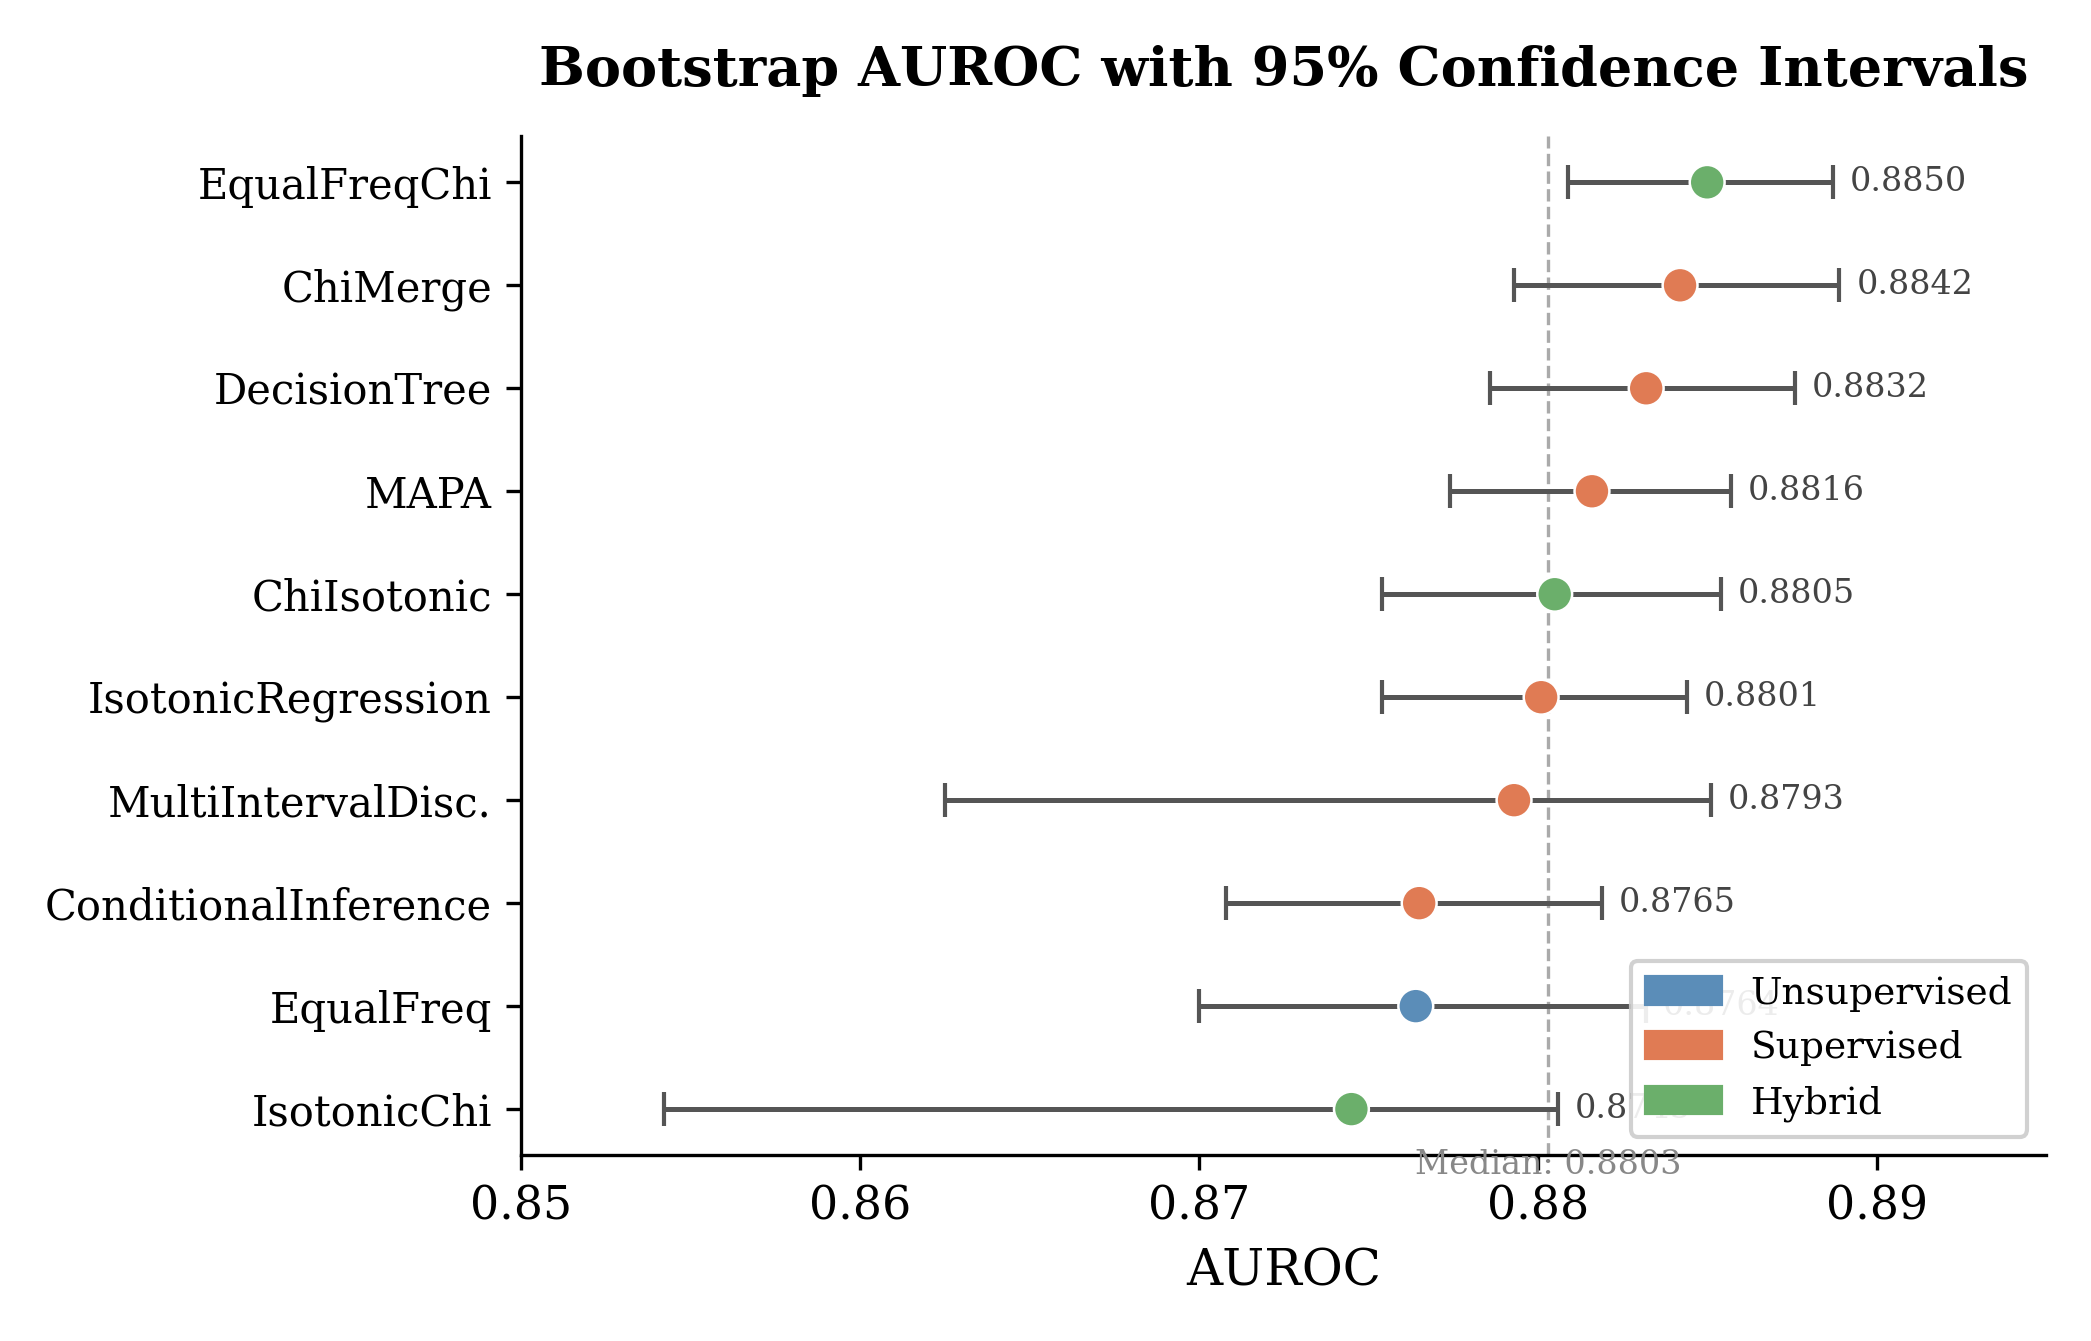
\includegraphics[width=0.65\textwidth]{fig1_auroc_forest.png}
    \caption{Forest plot of mean AUROC with 95\% bootstrap confidence intervals. Methods are sorted by mean AUROC. The dashed line indicates the median. Color indicates method category: blue (unsupervised), orange (supervised), green (hybrid).}
    \label{fig:auroc_forest}
\end{figure}

\FloatBarrier
\subsection{KS Statistic Performance}

\Cref{fig:ks_forest} shows the analogous forest plot for the KS statistic. The ranking differs from AUROC: Decision Tree leads with KS = 0.6136, followed by Isotonic Regression (0.6135) and EqualFreqChi (0.6135). This reshuffling reflects the different aspects of discrimination captured by AUROC (average across all thresholds) versus KS (maximum separation at a single threshold).

Notably, some methods that perform well on AUROC show relatively lower KS values (e.g., ChiMerge ranks 2nd on AUROC but 6th on KS), while others show the reverse (e.g., IsotonicRegression ranks 6th on AUROC but 2nd on KS). This metric disagreement underscores the importance of evaluating multiple performance measures.

\begin{figure}[htbp]
    \centering
    
\includegraphics[width=0.65\textwidth]{fig2_ks_forest.png}
    \caption{Forest plot of mean KS statistic with 95\% bootstrap confidence intervals. The ranking differs from AUROC, reflecting the different discrimination aspects captured by each metric.}
    \label{fig:ks_forest}
\end{figure}

\FloatBarrier
\subsection{Bootstrap Distribution Shapes}

\Cref{fig:auroc_violin} illustrates the full empirical distribution of AUROC values across the 1{,}000 bootstrap replicates as violin plots. Unlike the forest plots, which summarize the distribution via its mean and 95\% confidence interval bounds, the violin plots reveal the underlying density and shape of the performance variability. EqualFreqChi exhibits a compact, concentrated density map, visually confirming its tight stability. In contrast, methods like IsotonicChi display substantially wider and more diffuse distributions, underscoring their sensitivity to sampling variation across replicates.

\begin{figure}[htbp]
    \centering
    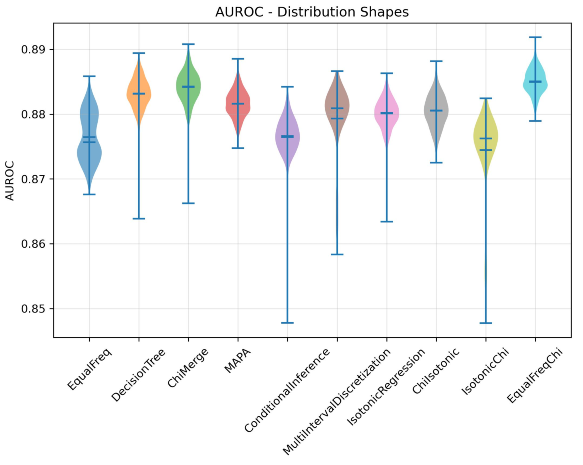
\includegraphics[width=0.65\textwidth]{fig6_Violin_auroc.png}
    \caption{Violin plots of AUROC distributions across 1{,}000 bootstrap replicates. The width of each violin represents the probability density of the performance metric, providing an expanded view of the resampling variability beyond standard error margins.}
    \label{fig:auroc_violin}
\end{figure}

\FloatBarrier
\subsection{Stability Analysis}

\Cref{fig:ci_width} presents the confidence interval widths for both AUROC and KS, sorted from widest (least stable) to narrowest (most stable). EqualFreqChi exhibits the narrowest CI width for both metrics (AUROC: 0.0078; KS: 0.0197), indicating that it produces the most consistent performance across bootstrap replicates. MAPA also shows excellent stability (AUROC: 0.0083; KS: 0.0217).

At the other extreme, IsotonicChi shows the widest CIs (AUROC: 0.0264; KS: 0.0556), indicating substantial variability. MultiIntervalDiscretization and EqualFreq also exhibit wide intervals. The stability ranking does not perfectly align with the performance ranking: DecisionTree, which ranks 3rd on AUROC, also achieves the 2nd-narrowest CI width (0.0090), making it an attractive choice that balances performance with stability.

\begin{figure}[htbp]
    \centering
    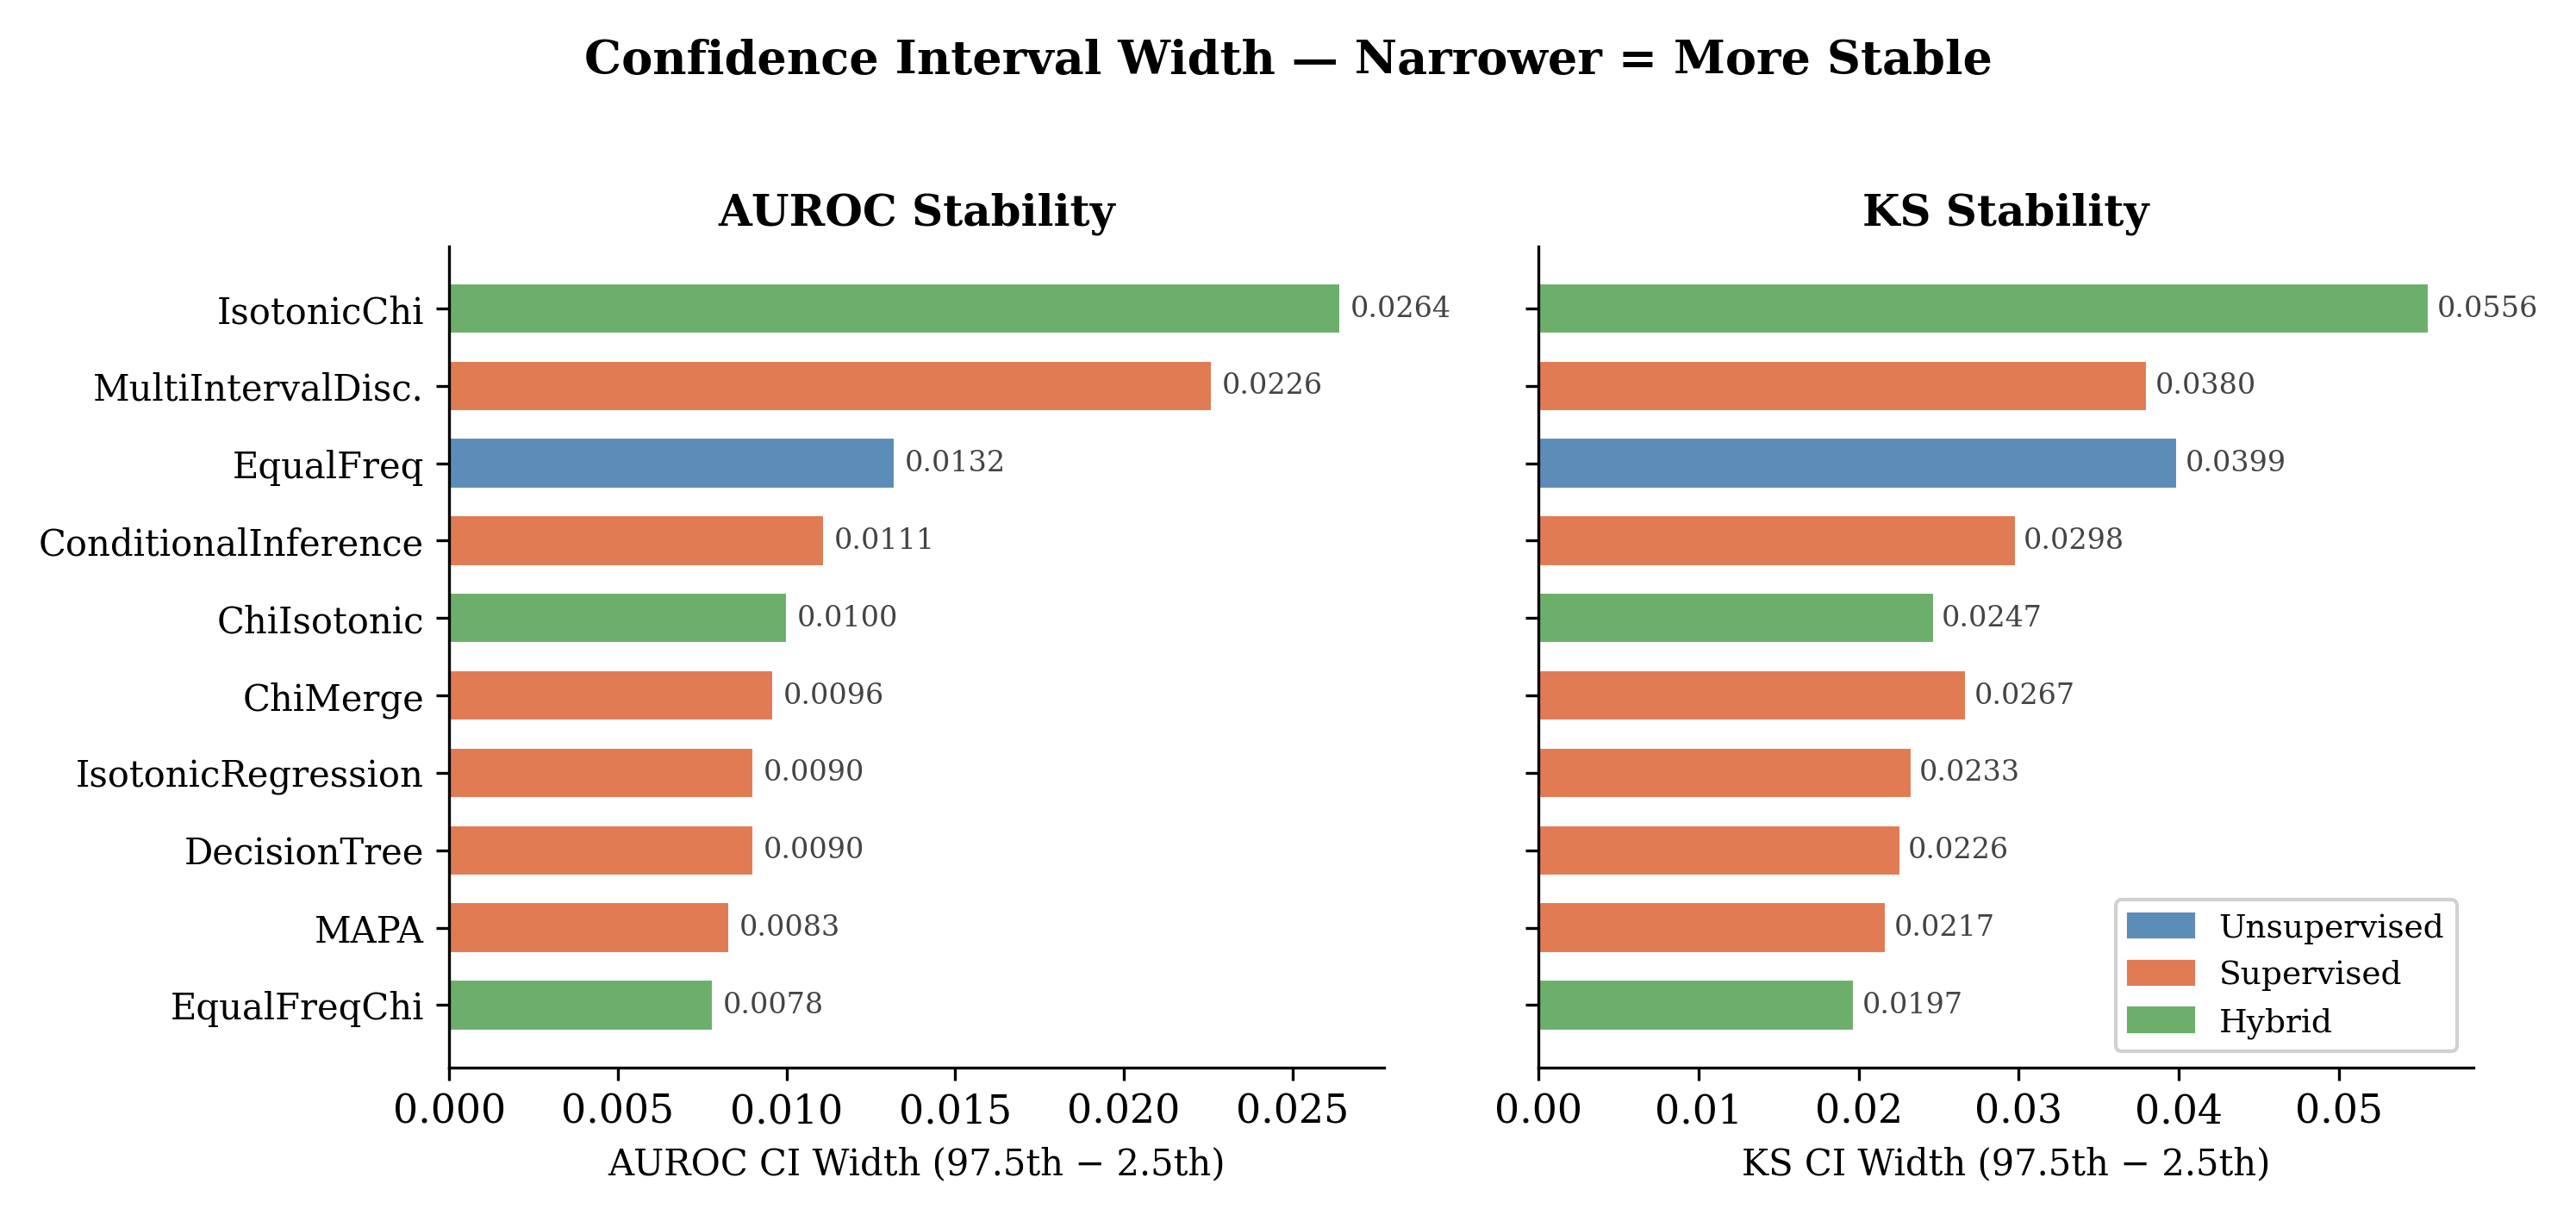
\includegraphics[width=0.85\textwidth]{fig3_ci_width_stability.png}
    \caption{Confidence interval widths for AUROC (left) and KS (right). Narrower bars indicate greater stability. EqualFreqChi achieves the narrowest intervals for both metrics, while IsotonicChi shows the highest variability.}
    \label{fig:ci_width}
\end{figure}

\FloatBarrier
\subsection{Multi-Metric Comparison}

\Cref{fig:scatter} provides a combined view of AUROC and KS performance with 2D error bars. Methods in the upper-right quadrant perform well on both metrics. EqualFreqChi occupies the best position, combining high AUROC with high KS and small error bars. The scatter plot also reveals the performance-stability trade-off: methods with larger error bars (e.g., IsotonicChi, MultiIntervalDisc.) may achieve reasonable mean performance but with substantially more variability.

\begin{figure}[htbp]
    \centering
    
\includegraphics[width=0.71\textwidth]{fig4_auroc_vs_ks_scatter.png}
    \caption{AUROC vs.\ KS statistic with 95\% confidence interval error bars. Numbered markers correspond to methods listed in the legend. Methods in the upper-right quadrant with tight error bars represent the best combination of performance and stability.}
    \label{fig:scatter}
\end{figure}

\FloatBarrier
\subsection{Pairwise Statistical Comparison}

\Cref{fig:ci_overlap_heatmap} presents the pairwise confidence interval overlap matrix for AUROC. This provides a complementary perspective to absolute magnitude comparisons by evaluating statistical distinguishability. Two methods whose 95\% confidence intervals overlap substantially cannot be considered statistically distinguishable at the 5\% level. EqualFreqChi and ChiMerge show extensive overlap with each other, indicating that within the top cluster, the methods perform similarly.

However, the top hybrid/supervised cluster is clearly distinguishable from the bottom-performing tier. EqualFreqChi shows no interval overlap with IsotonicChi, ConditionalInference, and other baseline methods. This provides strong graphical evidence that the hybrid strategy's performance advantage is genuine and not an artifact of random sampling variability.

\begin{figure}[htbp]
    \centering
    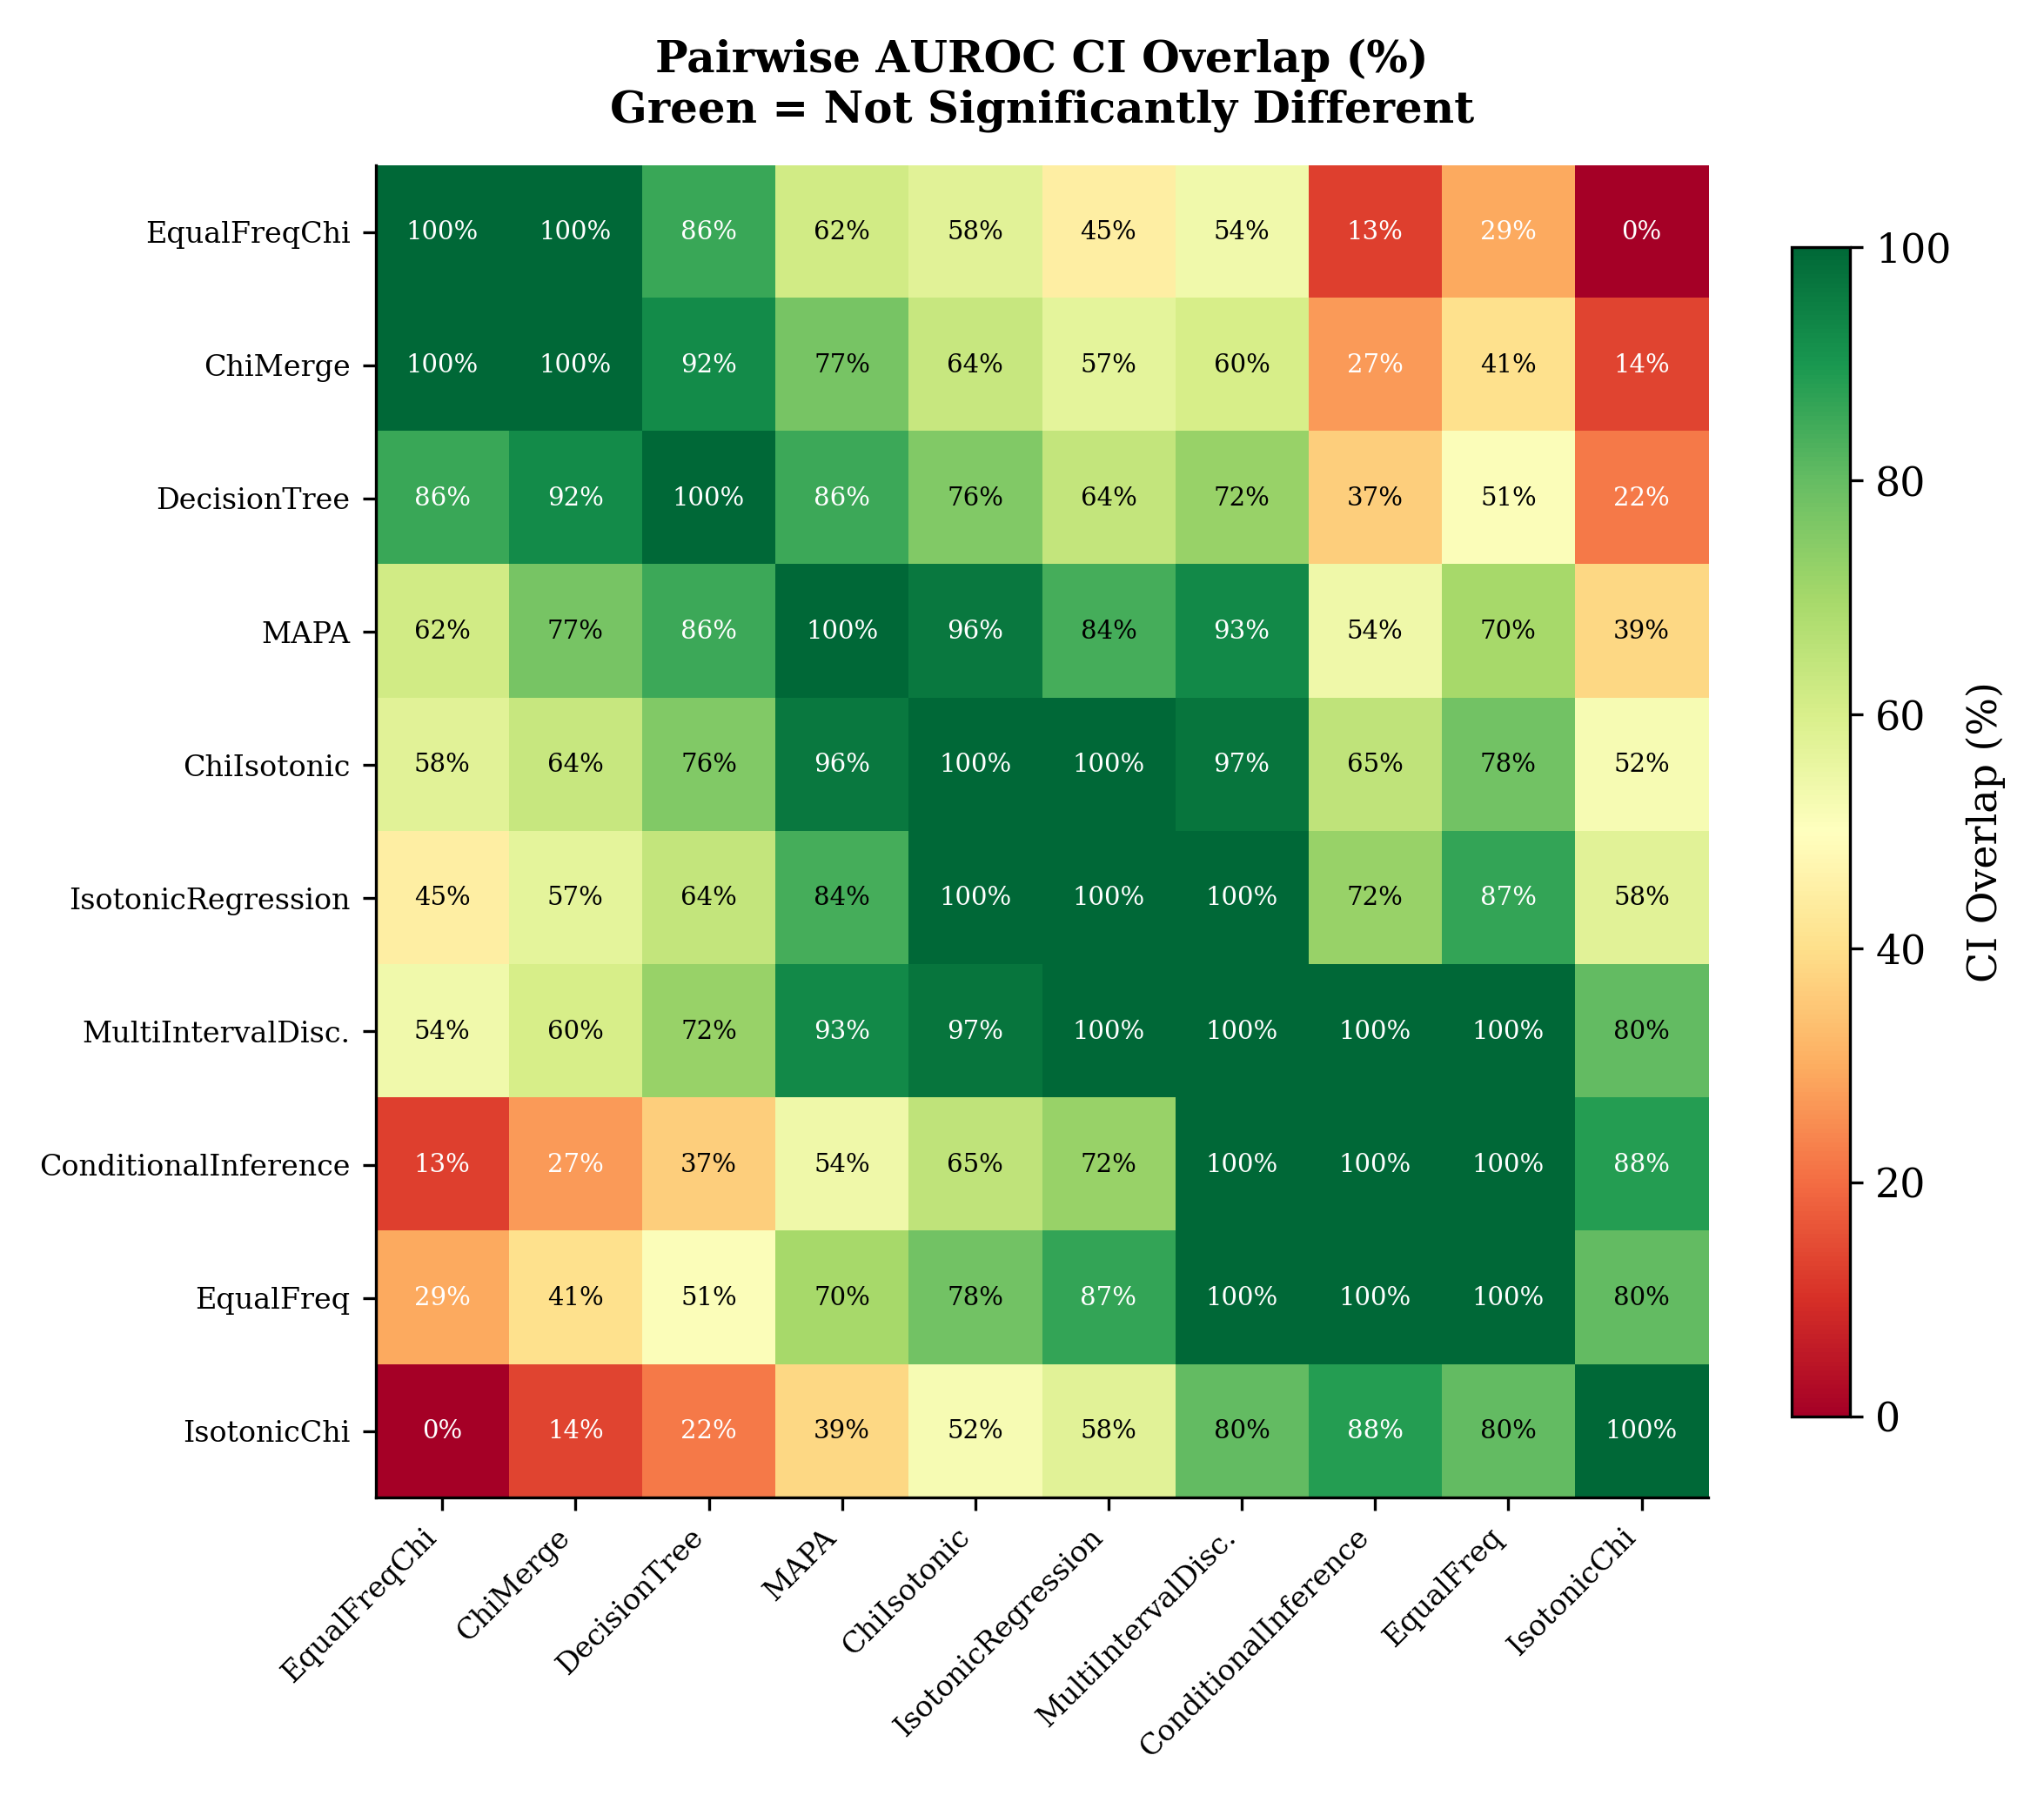
\includegraphics[width=0.95\textwidth]{fig5_ci_overlap_heatmap.png}
    \caption{Pairwise AUROC confidence interval overlap percentage. High values (green) indicate substantial overlap between strategy performance, while values near zero (red) denote statistically separated distributions. The top-performing cluster maintains clear separation from the lower ranks.}
    \label{fig:ci_overlap_heatmap}
\end{figure}

\FloatBarrier
% ============================================================================
\section{Discussion}
\label{sec:discussion}

\subsection{The Advantage of Hybrid Methods}

The most striking finding is the consistent superiority of EqualFreqChi, which combines equal-frequency initial binning with ChiMerge refinement. This hybrid approach achieves the best mean AUROC and the narrowest confidence intervals, dominating the other nine strategies on both performance and stability dimensions.

The mechanism behind this advantage is intuitive: equal-frequency binning provides a well-balanced initial partition that avoids the sparse-bin problems of purely supervised methods, while ChiMerge refinement merges bins that are statistically indistinguishable and sharpens the boundaries between bins that differ meaningfully. The result is a discretization that is both data-adaptive and statistically robust.

\subsection{The Supervised--Unsupervised Gap}

The sole unsupervised method (EqualFreq) ranks near the bottom on AUROC (9th of 10), confirming the well-established finding that incorporating target information during discretization improves classification performance \citep{dougherty1995supervised, garcia2013survey}. However, EqualFreq's deficit is modest---its mean AUROC (0.8764) is only 0.0086 below EqualFreqChi (0.8850)---suggesting that much of the model's discriminatory power comes from the logistic regression step and the underlying feature representations rather than the binning step alone.

\subsection{Metric Disagreement}

The different rankings produced by AUROC and KS highlight a known issue in model evaluation: no single metric captures all aspects of discriminatory performance \citep{hanley1982meaning}. AUROC summarizes discrimination across all thresholds, while KS focuses on the point of maximum separation. For credit scoring applications, where the operational threshold is often determined by business constraints, practitioners should evaluate both metrics and select strategies that perform well on both, as EqualFreqChi does.

\subsection{Stability as a Selection Criterion}

Perhaps the most practically relevant finding is the large variation in stability across methods. IsotonicChi's AUROC CI width (0.0264) is more than three times wider than EqualFreqChi's (0.0078). In production credit scoring systems, where models must perform consistently across different time periods and customer segments, stability is as important as average performance. A method that achieves slightly lower mean AUROC but with a much narrower confidence interval may be preferred in practice.

\subsection{Limitations}

Several limitations should be noted. First, the study uses a single credit dataset; generalizability to other datasets, industries, and outcome definitions remains to be established. Second, the binning algorithms are applied univariately; interactions between predictors are captured only through the logistic regression model, not through the discretization step. Third, all methods are evaluated under a common monotonicity constraint, which may favor some algorithms over others. Fourth, computational cost varies substantially across methods, and we do not formally evaluate the performance-cost trade-off.


% ============================================================================
\section{Conclusion}
\label{sec:conclusion}

This study provides a systematic comparison of ten monotonically enforced binning strategies for logistic regression in credit risk assessment. Using a 1{,}000-replicate bootstrap evaluation, we demonstrate that:

\begin{enumerate}[nosep]
    \item \textbf{EqualFreqChi} emerges as the top-performing strategy, achieving the highest AUROC (0.8850, 95\% CI: 0.8809--0.8887) and the narrowest confidence interval width (0.0078), indicating both superior discrimination and superior stability.
    \item \textbf{Hybrid strategies} that combine unsupervised initial binning with supervised refinement consistently outperform purely unsupervised or purely supervised approaches.
    \item \textbf{Stability varies substantially} across methods, with CI widths ranging from 0.0078 (EqualFreqChi) to 0.0264 (IsotonicChi)---a 3.4-fold difference that has significant practical implications for production systems.
    \item \textbf{AUROC and KS rankings differ}, underscoring the importance of multi-metric evaluation in binning strategy selection.
\end{enumerate}

These findings provide practitioners with empirically grounded guidance: when selecting a binning strategy for credit risk logistic regression, hybrid approaches---particularly EqualFreqChi---should be the default starting point. Future work should extend this analysis to multiple datasets, multivariate binning approaches, and the interaction between binning strategy and regularization in logistic regression.


% ============================================================================
\section{Reproducibility}
\label{sec:reproducibility}

To support transparency and enable independent verification of our findings, we document the full computational pipeline below.

\paragraph{Code Availability.} All ten binning algorithms, the feature encoding pipeline, monotonicity enforcement logic, and the bootstrap orchestration framework were manually implemented in Python~3.10. The complete source code is available at \url{https://github.com/USERNAME/binning-comparison} (to be populated upon publication). Logistic regression was implemented via scikit-learn (v1.3.0) \citep{pedregosa2011scikit}. No third-party binning libraries were used; each algorithm was implemented following the original specifications from the literature to ensure full control over the discretization process and reproducibility.

\paragraph{Bootstrap Configuration.} A total of 1{,}000 bootstrap replicates were executed. Each replicate drew a sample with replacement from the original dataset, applied a stratified 70/30 train--test split, and executed the full binning--encoding--modeling--evaluation pipeline independently for all ten strategies. Confidence intervals were computed as the 2.5th and 97.5th percentiles of the resulting bootstrap distributions.

\paragraph{Computational Resources.} The full bootstrap analysis was conducted on a high-performance computing node and required approximately 500 compute-hours. Peak memory usage reached 53.7\,GB due to the accumulation of per-iteration results across 1{,}000 replicates. Checkpointing was performed every 25 iterations to allow for fault-tolerant resumption.

\paragraph{Data Availability.} The credit dataset used in this study was provided by Equifax under a research agreement and is subject to data-use restrictions that prevent public redistribution. Researchers interested in replicating the analysis on comparable data may use publicly available credit datasets (e.g., the Kaggle ``Give Me Some Credit'' dataset or the UCI German Credit dataset) with the same pipeline.

\paragraph{Random Seed and Determinism.} Bootstrap sample indices were generated using NumPy's default PRNG with a fixed seed at the start of computation to ensure reproducibility. Due to the use of iterative optimization within some binning algorithms (e.g., isotonic regression, conditional inference), minor floating-point differences may arise across different hardware or library versions.


% ============================================================================
\bibliographystyle{plainnat}
\bibliography{references}



\end{document}
